\subsection{MNIST}
We compare the distribution of features computed over the MNIST training set 
to other datasets, including
the MNIST test set, samples generated with GANs and adversarial samples computed 
using FGSM. The training data is
scaled to $[0, 1]$ and the random baseline is sampled from a Bernoulli distribution with 
probability equal to the value of pixel intensities in the
MNIST training data, 0.13. Each GAN model is trained until the loss plateaus 
and the generated samples look similar to the real samples. The datasets
compared have 10 thousand samples each.

\begin{figure}[!h]
  \begin{center}
  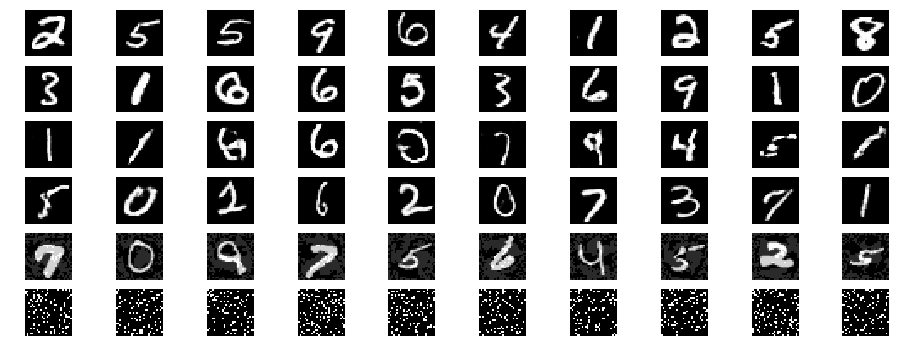
\includegraphics[width=0.8\linewidth]{mnist_samples.png}
  \caption{Samples drawn from MNIST train, test,
LSGAN, IWGAN, FSGM and Bernoulli respectively.}
  \label{fig:mnist_samples}
  \end{center}
\end{figure}

Visual inspection of the generated samples in
Figure~\ref{fig:mnist_samples} show that IWGAN seems to produce better samples
than LSGAN. Quantitatively, we use the MNIST training set as a reference and compare the
distribution of pixel intensities.  Table~\ref{tbl:mnist_pixel} reveals that
although samples generated with LSGAN and IWGAN look similar to the training
set, they are considerably different from the training set given the Kolgomorov-Smirnov (KS) Two
Sample Test and the Jensen-Shannon Divergence (JSD), specially if compared to
the same statistics on the MNIST test data. 

\begin{table}[!h]
\centering
\begin{tabular}{l|ll|l|}
                   & \multicolumn{2}{c|}{\cellcolor[HTML]{C0C0C0}KS Two Sample Test} & \multicolumn{1}{c|}{\cellcolor[HTML]{C0C0C0}JSD} \\
                   & Statistic   & P-Value   &                \\
mnist\_train       & 0.0         & 1.0       & 0.0            \\
mnist\_test        & 0.003177    & 0.0       & 0.000029       \\
mnist\_lsgan       & 0.808119    & 0.0       & 0.013517       \\
mnist\_iwgan       & 0.701573    & 0.0       & 0.014662       \\
mnist\_adversarial & 0.419338    & 0.0       & 0.581769       \\
mnist\_bernoulli   & 0.130855    & 0.0       & 0.0785009      
\end{tabular}
\caption{Statistical comparison over the distribution of pixel values for
different samples using MNIST training set as reference.}
\label{tbl:mnist_pixel}
\end{table}

These numerical phenomena can be understood by investigating the empirical CDFs 
in Figure~\ref{fig:mnist_pixel_ecdf}. The pixel values of the samples
generated with the GAN framework are mainly bi-modal and asymptotically
approach the modes of the distribution of pixel values in the real data, $0$ and $1$. Such behavior will be
present in any Generator trained using gradient descent and an asymptotically converging 
non-linearity, such as sigmoid and tanh, at the output of the generating function.

\begin{figure}[!h]
  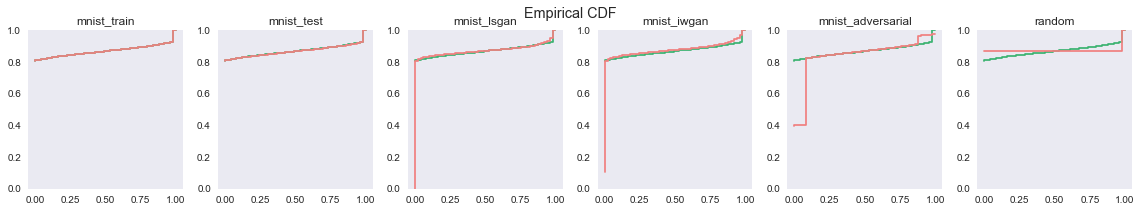
\includegraphics[width=\linewidth]{mnist_pixel_ecdf.png}
    \caption{Pixel empirical CDF of training data as reference (green) and other
    datasets(red)}
  \label{fig:mnist_pixel_ecdf}
\end{figure}

In addition, Figure~\ref{fig:mnist_pixel_distribution} shows that the GAN
generated samples smoothly approximate the modes of the distribution. This
smooth approximation is considerably different from the training and test sets.
Although these properties are not perceptually meaningful, they can be used to 
identify the source of the data, hence confirming hypotheses \ref{hyp:features}, 
\ref{hyp:visual} and \ref{hyp:difference}.

\begin{figure}[!h]
  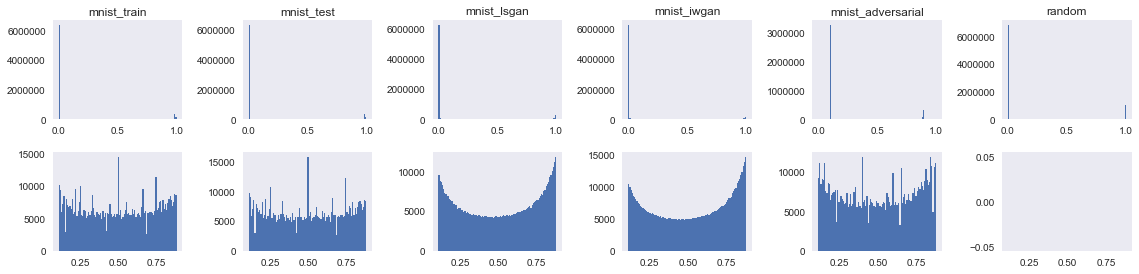
\includegraphics[width=\linewidth]{mnist_pixel_distribution.png}
  \caption{Histogram of pixel intensities for each dataset. First row shows
    histogram within the [0, 1] interval and 100 bins. Second row shows
    histograms between the [0.11, and 0.88] interval and 100 bins.}
  \label{fig:mnist_pixel_distribution}
\end{figure}

\subsection{Bach Chorales}
We investigate the properties of Bach chorales generated with the GAN framework
and verify if they satisfy musical specifications.
Bach chorales are polyphonic pieces of music, normally
written for 4 or 5 voices, that follow a set of
specifications/rules\footnote{The specifications define the characteristics of the 
musical style.}. For example, a global specification could assert that only a set of
durations are valid; a local specification could assert that only certain
transitions between states (notes) are valid depending on the current harmony.

For this experiment, we convert the dataset of Bach chorales to piano rolls. The
piano roll is a representation in which the rows represent note numbers, the columns
represent time steps and the cell values represent note intensities. We compare
the distribution of features computed over the training set, test set, GAN
generated samples and a random baseline sampled from a Bernoulli distribution with 
probability equal to the normalized mean value of intensities in the
training data. After scaling, the intensities in the training and test data are
strictly bi-modal and equal to $0$ or $1$. Figure~\ref{fig:chorales_samples} below
shows training, test, IWGAN and Bernoulli samples, thus confirming
hypothesis~\ref{hyp:generate}. Each dataset has roughly 1000 image patches.

\begin{figure}[!h]
  \begin{center}
  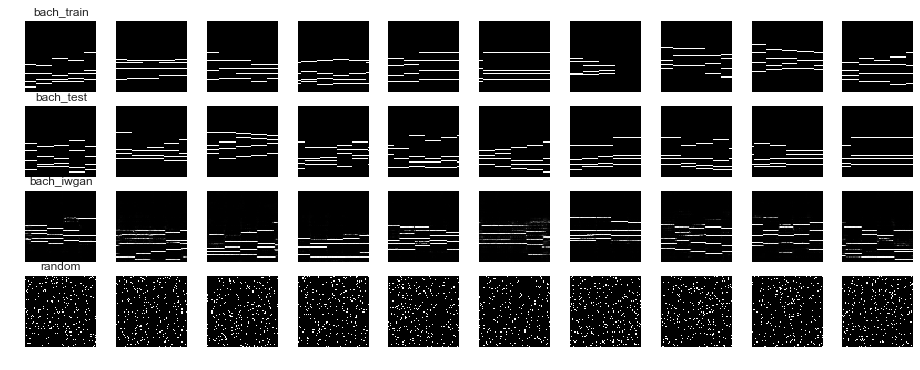
\includegraphics[width=0.8\linewidth]{chorales_samples.png}
  \caption{Samples drawn from Bach Chorales train, test,
IWGAN, and Bernoulli respectively.}
  \label{fig:chorales_samples}
  \end{center}
\end{figure}

Figure~\ref{fig:chorales_intensity_distribution} shows a behavior that is
similar to our previous MNIST experiments: the IWGAN asymptotically approximates
the modes of the distribution of intensity values. In the 
interest of space, we refer the reader to the online appendix\footnote{Not
provided to preserve anonymity} for statistics and other relevant information. 

\begin{figure}[!h]
  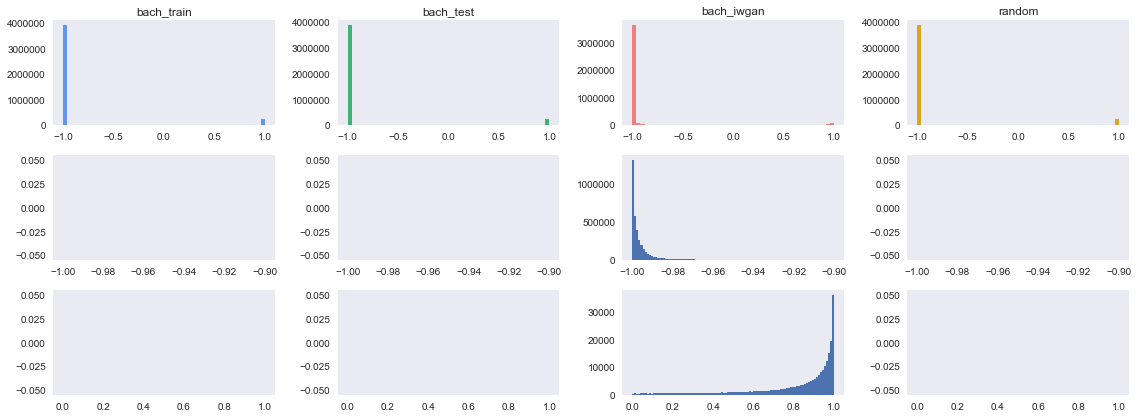
\includegraphics[width=\linewidth]{chorales_intensity_distribution.png}
  \caption{}
  \label{fig:chorales_intensity_distribution}
\end{figure}

Following, we investigate if the generated samples violate the specifications of
Bach chorales. For doing so, we first convert all datasets to boolean by 
thresholding at 0.5 such that values above the threshold are set to 1 or 0
otherwise. We use
these piano rolls to compute boolean Chroma~\cite{peeters2004large} feature and
to compute an empirical Chroma transition matrix, where the positive
entries represent existing and valid transitions. The transition matrix built on 
the training data is taken as the reference specification, i.e. anything that is 
not included is a violation of the specification. Table~\ref{tbl:chroma_violations}
shows the number of violations given each dataset. Although
Figure~\ref{fig:chorales_samples} shows generated samples that look similar to
the real data, the IWGAN samples have over 5000
violations, 10 times more than the test set! We use these facts to confirm
hypotheses \ref{hyp:features}, \ref{hyp:visual} and \ref{hyp:difference}.

\begin{table}[!h]
\centering
\begin{tabular}{lllll}
& \cellcolor[HTML]{C0C0C0}bach\_train & \cellcolor[HTML]{C0C0C0}bach\_test & \cellcolor[HTML]{C0C0C0}bach\_iwgan & \cellcolor[HTML]{C0C0C0}bach\_bernoulli \\ \cline{2-5} 
\multicolumn{1}{l|}{\cellcolor[HTML]{C0C0C0}Number of Violations} & 0                                   & 429                                & 5029                                & 58284                                  
\end{tabular}
\caption{Number of specification violations with training data as
    reference.}
\label{tbl:chroma_violations}
\end{table}

In addition to experiments with Chroma features, we computed the distribution of
note durations on the boolean piano roll described above.
Figure~\ref{fig:chorales_duration_distribution} shows the distribution of
note durations within each dataset. The train and test data are approximately
bi-modal and, again, the improved WGAN smoothly approximates the
dominating modes of the distribution. Table~\ref{tbl:duration} provides a numerical 
comparison between datasets.


\begin{figure}[!h]
    \begin{subfigure}[b]{0.65\textwidth}
        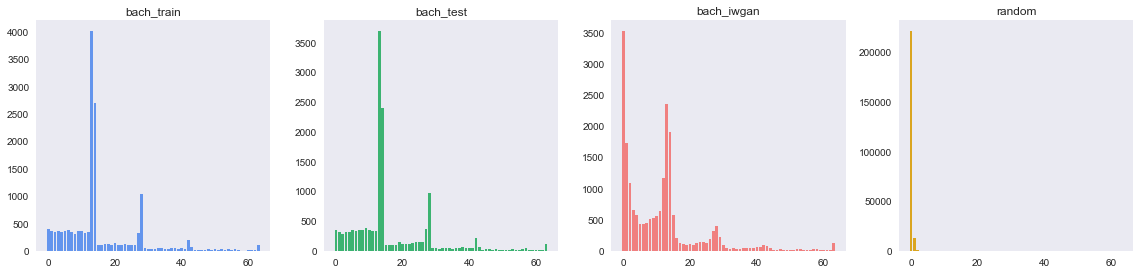
\includegraphics[width=\linewidth]{chorales_duration_distribution.png}
        \caption{Histogram of note durations}
        \label{fig:chorales_duration_distribution}
    \end{subfigure}
    \quad
    \begin{subfigure}[b]{0.3\textwidth}
    %\begin{table}[!h]
        \resizebox{1.0\textwidth}{!}{%
        \begin{tabular}{l|ll|l|}
                           & \multicolumn{2}{c|}{\cellcolor[HTML]{C0C0C0}KS Two Sample Test} & \multicolumn{1}{c|}{\cellcolor[HTML]{C0C0C0}JSD} \\
                           & Statistic   & P-Value  &         \\
        train       & 0.0          & 1.0      & 0.0     \\
        test        & 0.09375      & 0.929    & 0.002   \\
        iwgan       & 0.21875      & 0.080    & 0.084   \\
        bernoulli   & 0.93750      & 0.0      & 0.604   
        \end{tabular}
        }
        \caption{Test statistics}
        \label{tbl:duration}
    %\end{table}
    \end{subfigure}
\end{figure}

\subsection{Speech}
Within the speech domain, we investigate dynamic compressed Mel-Spectrogram 
samples produced with GANs trained on a subset of the NIST 2004 dataset, with
100 speakers. We divide the NIST 2004 dataset into training and test set,
generate samples with the GAN framework and use a random baseline sampled from 
a Exponential distribution with parameters chosen using heuristics.
The generated samples can be seen in
Figure~\ref{fig:speech_samples}, thus confirming hypothesis~\ref{hyp:generate}.
We obtain the Mel-Spectrogram by projecting a
spectrogram onto a mel scale, which we do with the python library
librosa~\cite{mcfee2015librosa}. More specifically,  we project the spectrogram 
onto 64 mel bands,
with window size equal to 1024 samples and hop size equal to 160 samples, i.e.
frames of 100ms long. Dynamic range compression is computed as described 
in~\cite{lukic2016speaker}, with $log(1 + C*M)$, where $C$ is the compression 
constant scalar set to $1000$ and $M$ is the matrix representing the Mel-Spectrogram.
Each dataset has approximately 1000 image patches and the GAN models are trained 
using DCGAN with the improved Wasserstein GAN algorithm.

\begin{figure}[!h]
  \begin{center}
  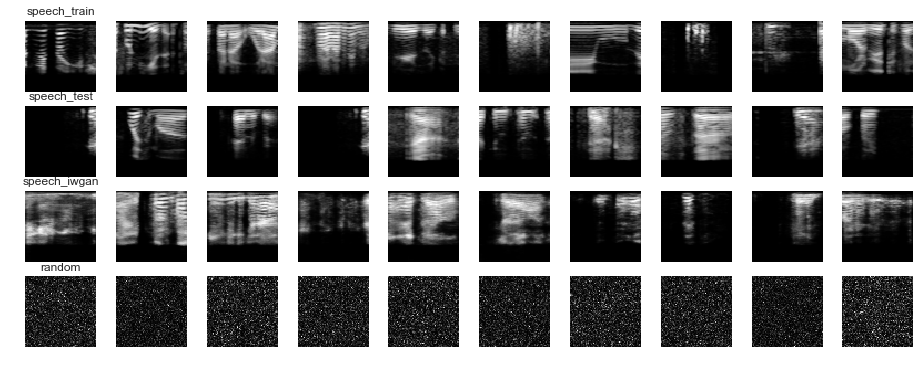
\includegraphics[width=0.8\linewidth]{speech_samples.png}
  \caption{Samples drawn from Mel-Spectrogram Speech train, test,
IWGAN, and exponential respectively.}
  \label{fig:speech_samples}
  \end{center}
\end{figure}

In Figure~\ref{fig:speech_intensity_ecdf} we show the empirical CDFs of intensity
values. Unlike our previous experiments where intensity (Bach Chorales)
or pixel value (MNIST) was linear, in this experiment intensities are compressed using the
log function. This considerably reduces the distance between the empirical CDFs
of the training data and GAN samples,
specially around the saturating points of the tanh non-linearity, $-1$ and $1$ in this
case. In Table~\ref{tbl:speech_intensity} we show numerical analysis of the
differences and confirm hypotheses \ref{hyp:features} and \ref{hyp:visual}.
\begin{figure}[!h]
    \begin{subfigure}[b]{0.65\textwidth}
        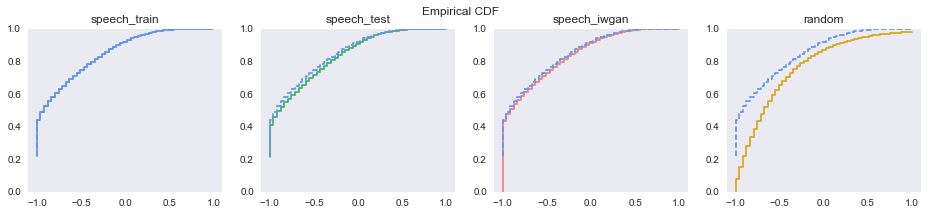
\includegraphics[width=1.0\linewidth]{speech_intensity_ecdf.png}
        \caption{Intensity empirical CDF of training data in blue
        and other datasets.}
        \label{fig:speech_intensity_ecdf}
    \end{subfigure}
    \quad
    \begin{subfigure}[b]{0.3\textwidth}
    %\begin{table}[!h]
        \resizebox{1.0\textwidth}{!}{%
        \begin{tabular}{l|ll|l|}
                           & \multicolumn{2}{c|}{\cellcolor[HTML]{C0C0C0}KS Two Sample Test} & \multicolumn{1}{c|}{\cellcolor[HTML]{C0C0C0}JSD} \\
                    & Statistic    & P-Value  &         \\
        train       & 0.0          & 1.0      & 0.0     \\
        test        & 0.03685      & 0.0      & 0.00080   \\
        iwgan       & 0.22149      & 0.0      & 0.00056   \\
        bernoulli   & 0.36205      & 0.0      & 0.11423   
        \end{tabular}
        }
        \caption{Test statistics}
        \label{tbl:speech_intensity}
    %\end{table}
    \end{subfigure}
    \caption{Empirical CDF and statistical tests of speech intensity}
    \label{fig:speech_intensity}
\end{figure}

Figure~\ref{fig:speech_moments} shows the distribution of statistical moments computed on
spectral centroids and slope. The distributions from different sources
considerably overlap, indicating that the generator has efficiently approximated
the real distribution of these features.

\begin{figure}[!h]
    \centering
    \begin{subfigure}[b]{0.45\textwidth}
        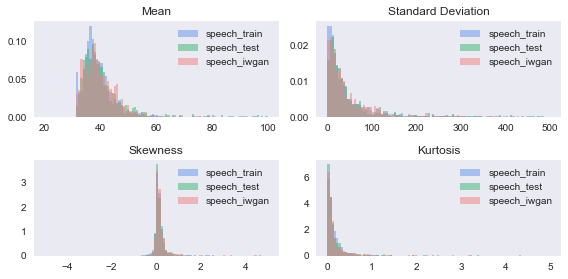
\includegraphics[width=\linewidth]{speech_spectral_centroid_moments.png}
        \caption{Spectral Centroid Moments}
        \label{fig:speech_spectral_centroid_moments}
    \end{subfigure}
    \quad
    \begin{subfigure}[b]{0.45\textwidth}
        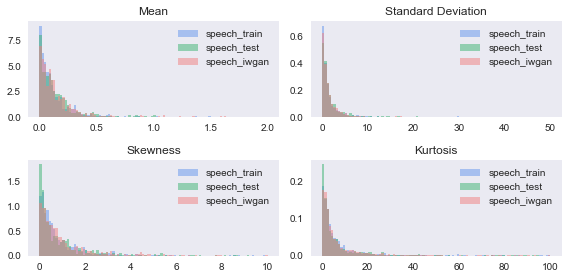
\includegraphics[width=\linewidth]{speech_spectral_slope_moments.png}
        \caption{Spectral Slope Moments}
        \label{fig:speech_spectral_slope_moments}
    \end{subfigure}
    \caption{Moments of spectral centroid (left) and slope(right)}
    \label{fig:speech_moments}
\end{figure}

Figure~\ref{fig:speech_spectral_stats} shows statistics used to compare the
reference (training data) and other datasets. The difference between
KS-Statistics and JSD of the test data and generated samples are negligible.
Interestingly, the p-values of the spectral slope of the improved WGAN are considerably
higher than the test data. For these reasons and although 
Table~\ref{tbl:speech_intensity} shows a significant difference between the 
KS-Statistic of test data and generated data with respect to the training
data, we refrain from confirming hypothesis \ref{hyp:difference}. An adversary
can easily manipulate the generated data to considerably decrease 
this difference and still keep the high similarity in features harder to
simulate such as moments of spectral centroid or slope. 

\begin{figure}[!h]
    \centering
    \begin{subfigure}[b]{.45\textwidth}
        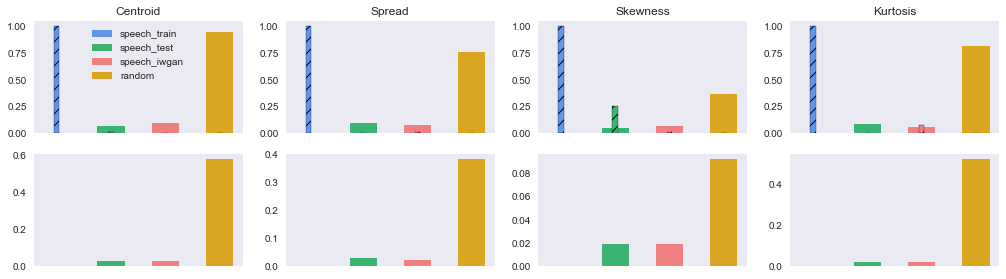
\includegraphics[width=\linewidth]{speech_spectral_centroid_stats.png}
        \caption{Spectral Centroid Statistics}
        \label{fig:speech_spectral_centroid_stats}
    \end{subfigure}
    \quad
    \begin{subfigure}[b]{.45\textwidth}
        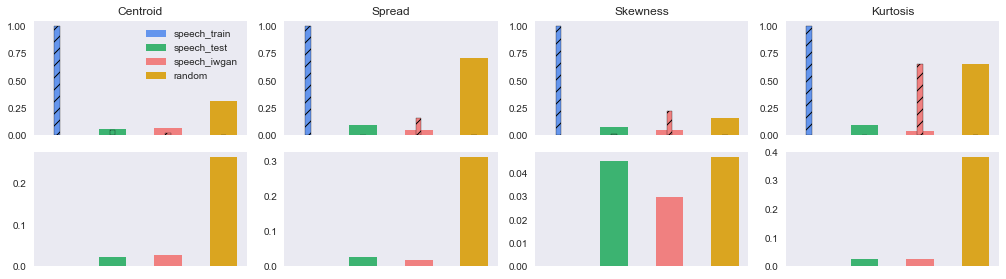
\includegraphics[width=\linewidth]{speech_spectral_slope_stats.png}
        \caption{Spectral Slope Statistics}
        \label{fig:speech_spectral_slope_stats}
    \end{subfigure}
    \caption{Statistics of spectral centroid (left) and slope(right)}
    \label{fig:speech_spectral_stats}
\end{figure}
